\documentclass[usenames,dvipsnames,handout]{beamer}

\usepackage{tikz}
\usepackage{tkz-berge}
\usepackage{tkz-graph}
\usepackage{subcaption}

\usetikzlibrary{patterns,arrows,decorations.pathreplacing}

\usepackage{xcolor}
\definecolor{dblue}{RGB}{20,66,129}
\definecolor{rose}{RGB}{255,101,122}
\definecolor{crimsonred}{RGB}{132,22,23}
\definecolor{darkblue}{RGB}{72,61,139}

\definecolor{deepblue}{RGB}{36,123,160}
\definecolor{deepred}{RGB}{255,22,84}
\definecolor{deeporange}{RGB}{240,111,62}

\definecolor{olive}{rgb}{0.3, 0.4, .1}
\definecolor{fore}{RGB}{249,242,215}
\definecolor{back}{RGB}{51,51,51}
\definecolor{title}{RGB}{255,0,90}
\definecolor{dgreen}{rgb}{0.,0.6,0.}
\definecolor{gold}{rgb}{1.,0.84,0.}
\definecolor{JungleGreen}{cmyk}{0.99,0,0.52,0}
\definecolor{BlueGreen}{cmyk}{0.85,0,0.33,0}
\definecolor{RawSienna}{cmyk}{0,0.72,1,0.45}
\definecolor{Magenta}{cmyk}{0,1,0,0}


\DeclareMathOperator{\RR}{\textbf{R}}
\DeclareMathOperator{\QQ}{\textbf{Q}}
\DeclareMathOperator{\ZZ}{\textbf{Z}}
\DeclareMathOperator{\TT}{\mathbf{T}}
\DeclareMathOperator{\PP}{\mathbf{P}}
\DeclareMathOperator{\EE}{\mathbf{E}}
\DeclareMathOperator{\fordim}{\text{dim}_{\textbf{F}}}
\DeclareMathOperator{\hausdim}{\text{dim}_{\textbf{H}}}
\DeclareMathOperator{\minkdim}{\text{dim}_{\textbf{M}}}
\DeclareMathOperator{\lowminkdim}{\text{\underline{dim}}_{\textbf{M}}}

\title{Salem Sets Avoiding Nonlinear Patterns}
\author{Jacob Denson}
\institute{}

\begin{document}

\maketitle




\begin{frame}
    \frametitle{General Research Question}

    \begin{center}
    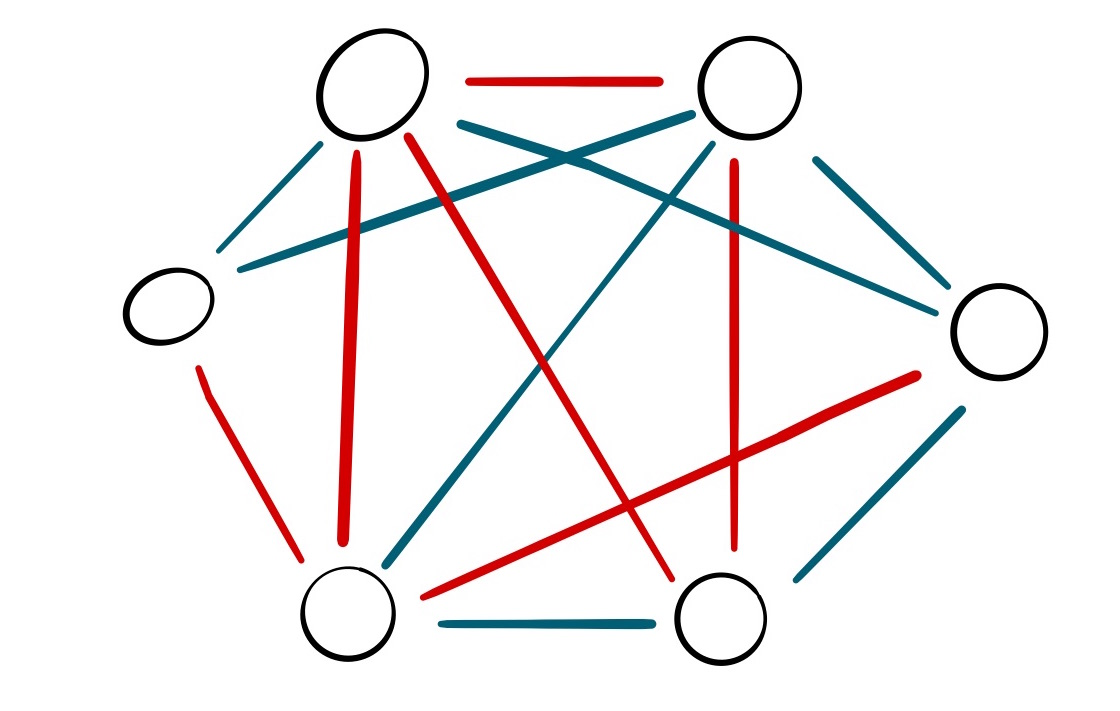
\includegraphics[width=0.4\textwidth]{../Images/RamseyTheory}
    \end{center}

    \begin{itemize}
        \item Phenomenon: Structure appears in suitably large objects.

        \item Like Ramsey Theory, but with a more analytical foundation, e.g. Geometric Measure Theory / Harmonic Analysis.
    \end{itemize}
\end{frame}





\begin{frame}
  \frametitle{Examples}

\begin{tabular}{p{0.8\textwidth}p{0.3\textwidth}}

\begin{itemize}
    \pause
    \item How large can a subset $X$ of $\RR^d$ be such that there does not exist four distinct points $x_1,x_2,x_3,x_4 \in X$ which form a parallelogram, i.e. satisfy $x_2 - x_1 = x_4 - x_3$.

    \pause
    \item How large can a subset $X$ of $\RR^d$ be such that no three distinct points $x_1,x_2,x_3 \in X$ form a right angle, i.e satisfy $(x_2 - x_1) \cdot (x_3 - x_1) = 0$.

    \item How large can a subset of $\RR^d$ be, such that the distances between any two points is irrational?

%    \pause
%    \item How large can an additive group $G \subset \RR^d$ be, such that $G \cap \QQ^d = \{ 0 \}$.

%    \pause
%    \item Given any function $f: X \times \dots X \to \RR$, how large can a set $X \subset \RR^d$ be such that for any distinct $x_1, \dots, x_n \in X$, $f(x_1, \dots, x_n) \neq 0$.
\end{itemize}

\end{tabular}
\end{frame}





\begin{frame}

\begin{itemize}
    \item The problem isn't well posed for these patterns
    \begin{itemize}
        \item If $S \subset \RR^d$ has positive measure, it cannot avoid these patterns.
        \item We can find discrete sets of arbitrarily large cardinality avoiding these patterns.
        \item Need a measure of size `between' cardinality and Lebesgue measure.
    \end{itemize}
\end{itemize}

\end{frame}






\begin{frame}
  \frametitle{Fractional Dimension}

\begin{itemize}
    \item<1-> \emph{Fractional dimensions} measure largeness / thickness of sets. Standard fractional dimension are defined in terms of coverings.
    %
    \begin{itemize}
        \item Roughly speaking, a set $X \subset \RR^d$ has \emph{Minkowski dimension} $s$ if it can be covered by at most $r^{-s}$ balls of radius $r$, for arbitrarily small $r > 0$.



%        \item Again working roughly, a set $X \subset \RR^d$ has \emph{Hausdorff dimension} $s$ if it can be covered by a family of arbitrarily small balls $\{ B_1(r_1), B_2(r_2),\dots \}$, where $\sum_{i = 1}^\infty r_i^s < \infty$.
    \end{itemize}
    %
    \item If $|X| > 0$, $\hausdim(X) = \lowminkdim(X) = d$.

    \item If $\#(X) < \infty$, $\hausdim(X) = \lowminkdim(X) = 0$.
\end{itemize}

\end{frame}







\begin{frame}
    \frametitle{Fourier Dimension}

\begin{itemize}
    \item<3-> A compact set $X$ has \emph{Fourier dimension} at least $s$ if there exists a Borel probability measure $\mu$ supported on $X$ such that
    %
    \[ |\widehat{\mu}(\xi)| \lesssim |\xi|^{-s/2} \]
    %
    for $\xi \in \RR^d$. Then $\fordim(X)$ is the supremum of such values $s$.

%    \item<4-> Poisson summation implies
    %
%    \[ \sup_{\xi \in \RR^d} |\widehat{\mu}(\xi)| |\xi|^{s/2} \lesssim \sup_{\xi \in \ZZ^d} |\widehat{\mu}(\xi)| |\xi|^{s/2}, \]
    %
%    so we need only look at integer valued frequencies.

    \item If $s < \hausdim(X)$, then $|\widehat{\mu}(\xi)| |\xi|^{s/2}$ is small for \emph{most} $\xi$, i.e.
    %
    \[ \frac{| \{ \xi \in B_R: |\widehat{\mu}(\xi)| \geq |\xi|^{-s/2} \}|}{|B_R|} = o(1). \]
    %
    But a uniform bound is not always possible.

    \item In general $\fordim(X) \leq \hausdim(X) \leq \minkdim(X)$.

%    \item<5-> A useful heuristic (which isn't always sufficient depending on the definition of fractal dimension used) is that a set has fractal dimension at most $s$ if it can be covered by $O(r^{-s})$ balls of radius $r$.

%    \item<4-> Hausdorff dimension $\approx$ Minkowski dimension.
\end{itemize}

%\visible<3->{
%    \begin{center}
%        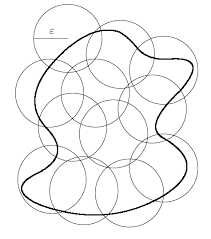
\includegraphics[width=0.3\textwidth]{../Images/CoveringNumber}
%    \end{center}
%}

\end{frame}

\begin{frame}
    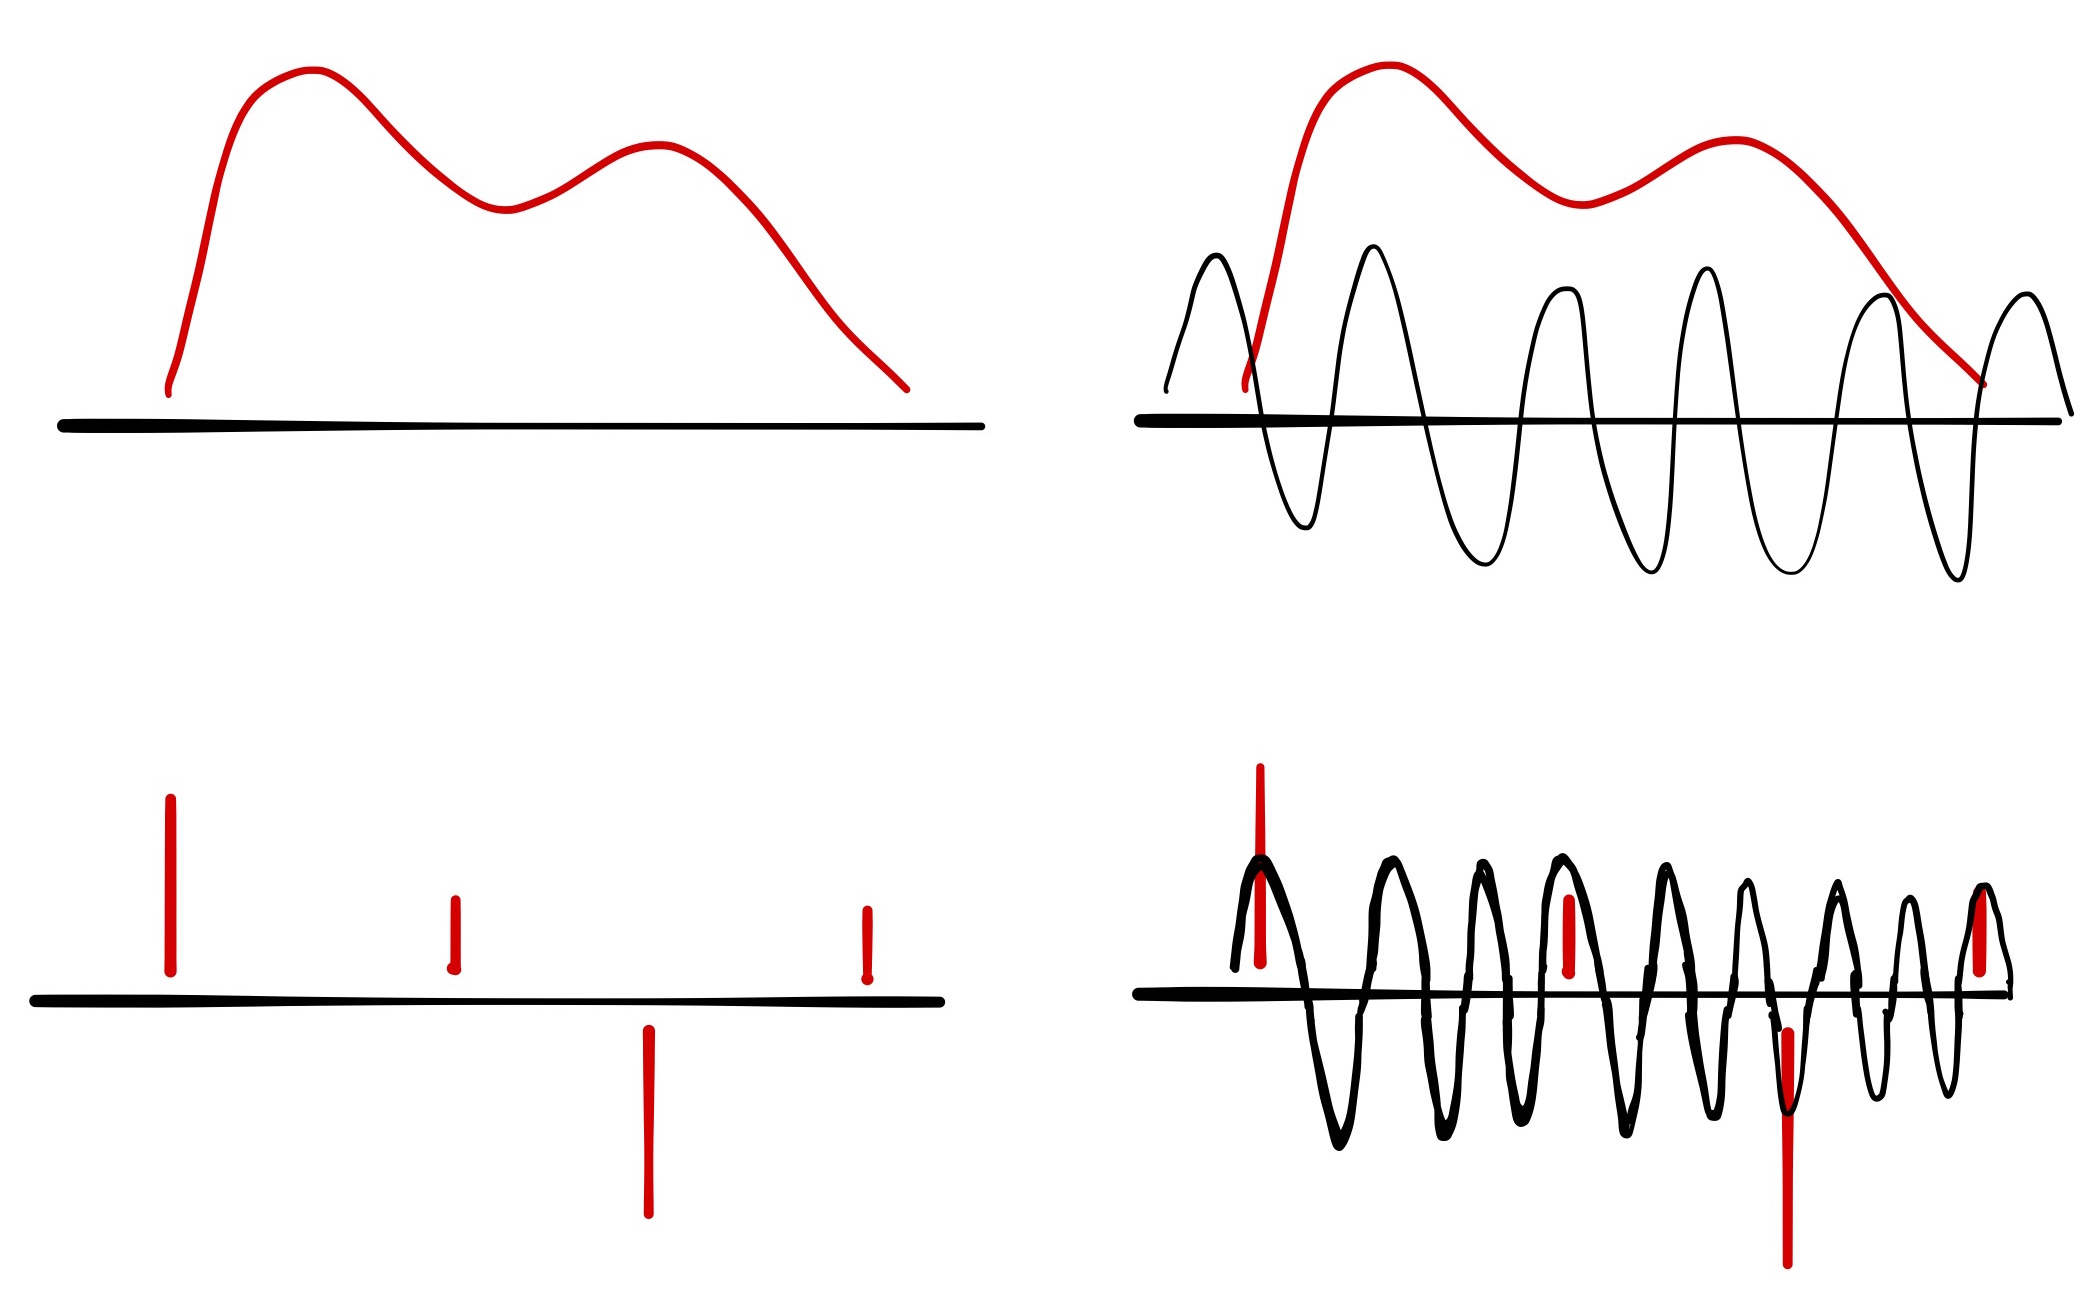
\includegraphics[width=\textwidth]{../Images/FourierDimension}
\end{frame}




\begin{frame}
    \frametitle{An Example}

    \begin{itemize}
        \item Let $C$ be the middle thirds Cantor set.

        \item For each $n$, $C$ is covered by $2^n$ intervals of length $1/3^n$.

        \item Recall a set has Minkowski dimension $s$ if it can be covered by $r^{-s}$ intervals of length $r$. Here $r = 1/3^n$, and
        %
        \[ 2^n = 3^{n \log_3 2} = r^{- \log_3 2}. \]
        %
        This suggests that $\hausdim(C) = \minkdim(C) = \log_3 2 \approx 0.63$.

        \item On the other hand, $\fordim(C) = 0$, since $C$ is highly correlated with waves of frequency $3^n$.
    \end{itemize}

        \begin{center}
    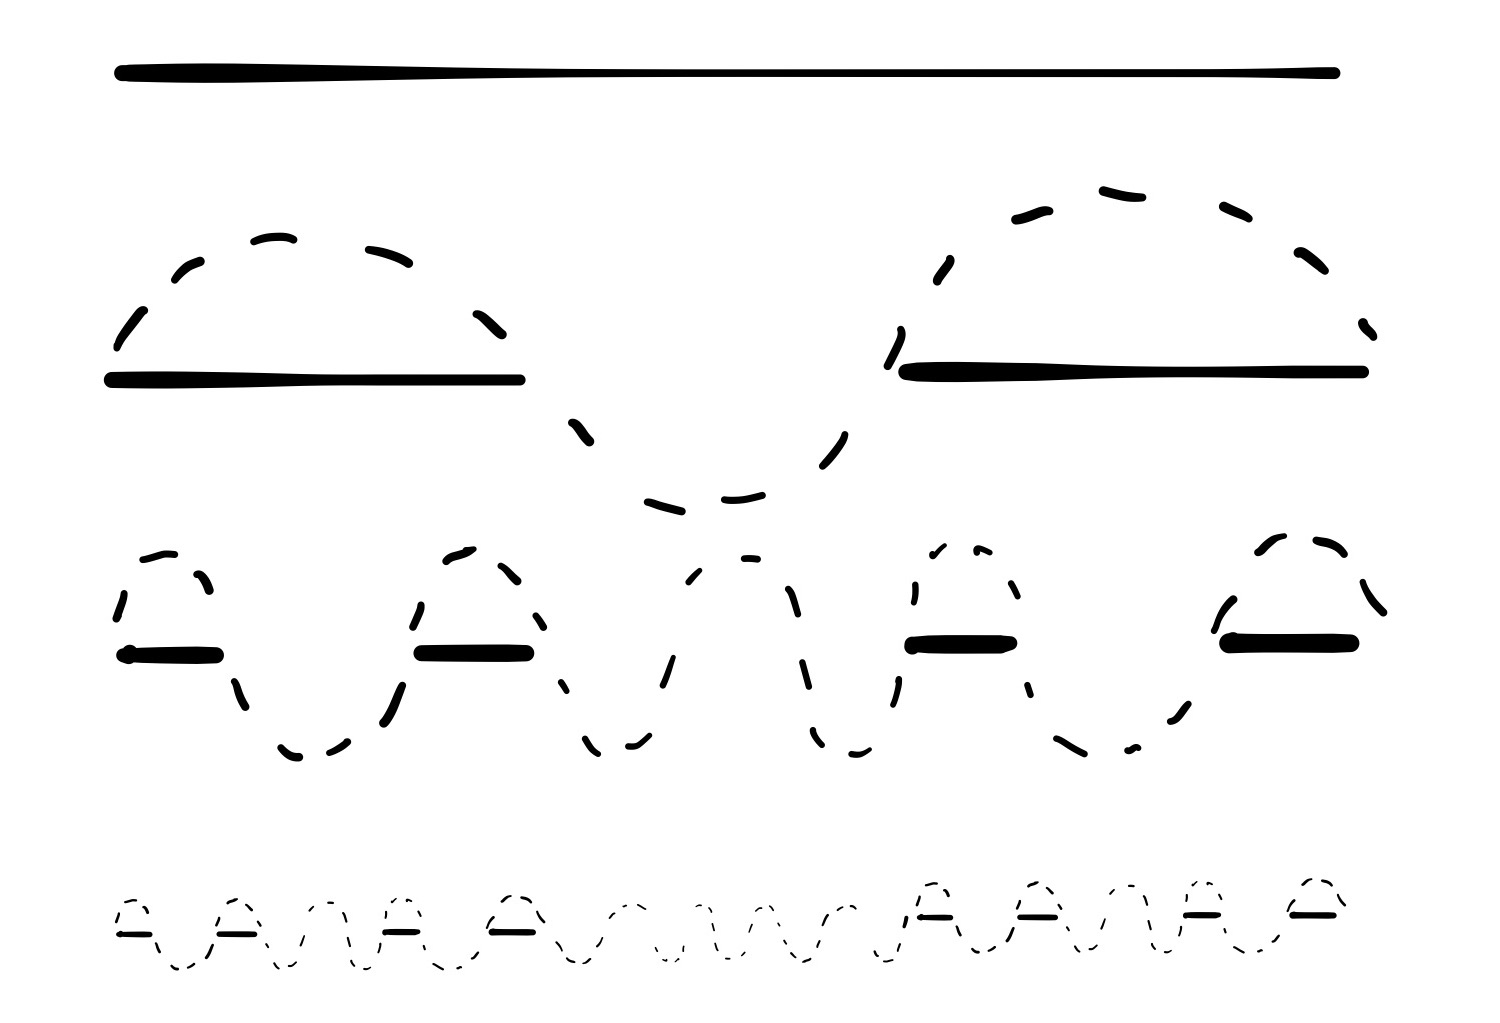
\includegraphics[width=0.5\textwidth]{../Images/CantorSetFourier}
    \end{center}
\end{frame}





\begin{frame}
    \frametitle{Salem Sets}

    \begin{itemize}
        \item If, at each stage of the Cantor set construction, instead of taking the middle third $J$ from each length $l$ interval $I$, we remove $l \cdot t_I + J$, where $t_I \in [-1/6,1/6]$ is selected uniformly at random, then we find that
        %
        \[ \fordim(X) = \hausdim(X) = \minkdim(X) = \log_3 2. \]

        \item A set is \emph{Salem} if $\fordim(X) = \hausdim(X)$.

        \item Main Focus of Talk: To construct Salem sets, the more probabilistic tools we can develop (especially concentration of measure / square root cancellation results) the better.
    \end{itemize}
\end{frame}





\begin{frame}
    Now Let's Return to Pattern Avoidance
\end{frame}




\begin{frame}
    \frametitle{The General Problem}

    \begin{itemize}
        \item {\bf Avoidance Problem}: Given a set $Z \subset \mathbf{R}^{nd}$, find $X \subset \mathbf{R}^d$ with large \emph{Fourier} dimension such that for distinct points $x_1, \dots, x_n \in X$, $(x_1, \dots, x_n) \not \in Z$. We say $X$ \emph{avoids} $Z$.

        \pause
        \item Let $Z = \{ (x,y,z) \in (\RR^d)^3: (x - z) \cdot (y - z) = 0 \}$.
        %
        \begin{itemize}
            \item $X \subset \RR^d$ avoids $Z$ iff $X$ does not contain any right angles.
        \end{itemize}

        \pause
        \item For each $m \in \ZZ^n - \{ 0 \}$ and $a \in \ZZ$, define
        %
        \[ Z(m,a) = \{  (x_1, \dots, x_n) \in (\RR^d)^n : m_1x_1 + \dots + m_nx_n = a \}. \]
        %
        \pause
        If $Z_n = \bigcup_{m \in \ZZ^n - \{ 0 \}} \bigcup_{a \in \ZZ} Z(m,a)$, then $X \subset \RR^d$ avoids $Z_n$ for all $n > 0$ if and only if $X$ generates a subgroup of $\RR^d$ disjoint from $\QQ^d - \{ 0 \}$.

    \end{itemize}
\end{frame}





\begin{frame}
    \begin{itemize}
        \pause
        \item Fourier Dimension often gives much more structural information about a set than Minkowski dimension does.

        \pause
        \item (Keleti, 1998) There exist an `independant' set $X \subset \RR$ with $\hausdim(X) = 1$ such that there exists no nontrivial solutions to $m_1x_1 + \dots + m_nx_n = 0$ for any $m \in \ZZ^n$ and $x_1, \dots, x_n \in X$.

        \pause
        \item (Rudin, 1960) If $\fordim(X) \geq 1/n$, then there exists some $m \in \ZZ^n$ and some $x_1, \dots, x_n \in X$ such that $m_1 x_1 + \dots + m_n x_n = 0$.
    \end{itemize}
\end{frame}


\begin{frame}
    \begin{itemize}
        \pause
        \item (K\"{o}rner, 2009) There exists a Salem set $X$ with $\fordim(X) = 1/(n-1)$ that contains no solutions to $m_1x_1 + \dots + m_nx_n = 0$ for any $m \in \ZZ^n$.

        \pause
        \item (Schmerkin, 2015) There exists a Salem set $X$ with $\fordim(X) = 1$ that contains no three term arithmetic progressions, i.e. no nontrivial solutions to the equation $x_2 - x_1 = x_3 - x_2$.

        \pause
        \item (Liang and Pramanik, 2019) There exists a Salem set $X$ with $\fordim(X) = 1$ that contains no solutions to a `translation invariant' equation of the form $m_1x_1 + \dots + m_n x_n = m_0 x_0$, where $m_0,\dots,m_n \geq 0$ and $m_1 + \dots + m_n = m_0$.
    \end{itemize}
\end{frame}


\begin{frame}
    \frametitle{Results in Literature}

    \begin{itemize}
        \item How does the geometry of $Z$ help us?
    \end{itemize}

    \begin{center}
    \begin{tabular}{| p{4cm} | p{4cm} | p{1.5cm} |}
        \hline
        Author & Geometry of $Z$ & $\hausdim(X)$\\
        \hline
        Math\'{e} (2012) & A degree $r$ algebraic hypersurface in $\RR^{dn}$ & $d/r$\\
        \hline
        Fraser and Pramanik (2016) & An $nd - m$ dimensional surface in $\RR^{dn}$ & $\frac{m}{n-1}$\\
        \hline
        Denson, Pramanik, and Zahl (2019) & A subset of $\RR^{dn}$ with (lower) Minkowski dimension $s$ & $\frac{dn - s}{n - 1}$\\
        \hline
        Denson (2019) & A subset of $\RR^n$ such that there exists a full rank linear map $\pi: \RR^n \to \RR^m$ where $\pi(Z)$ is $s$ dimensional & $\frac{m - s}{m}$\\
        \hline
    \end{tabular}
    \end{center}

    \begin{itemize}
        \item Can we modify these constructions to obtain Salem sets?
    \end{itemize}
\end{frame}







\begin{frame}
    \frametitle{Salem Set Result}

    \pause
    \begin{theorem}
        If $Z$ is a countable union of sets with (lower) Minkowski dimension bounded by $s$, we can find a Salem set $X$ avoiding $Z$ with
        %
        \[ \fordim(X) = \frac{nd - s}{n - 1/2}. \]
    \end{theorem}

    \begin{itemize}
        \item The previous results find a set $X$ with
        %
        \[ \hausdim(X) = \frac{nd - s}{n - 1}. \]
    \end{itemize}
\end{frame}




\begin{frame}
    \frametitle{Salem Set Result}

    \pause
    \begin{theorem}
        If $Z$ is a countable union of sets of the form
        %
        \[ \{ (x_1,\dots,x_n) \in \RR^{dn} : x_n = f(x_1,\dots,x_{n-1}) \} \]
        %
        where $f: \RR^{d(n-1)} \to \RR^d$ is smooth, and the matrix $D_{x_k} f(x_1,\dots,x_{n-1}) = \left( \frac{\partial f^i}{\partial x_{kj}} \right)$ is invertible for each $k$ and distinct $x_1,\dots,x_n \in \RR^d$, then we can find a Salem set $X$ avoiding $Z$ with
        %
        \[ \fordim(X) = \frac{d}{n - 3/4}. \]
    \end{theorem}

    \begin{itemize}
        \item The previous results find a set $X$ with $\hausdim(X) = \frac{d}{n - 1}$.

        \item We will focus on the ideas behind this proof in this talk.
    \end{itemize}
\end{frame}









\begin{frame}
    \frametitle{Applications}

    TODO

%    \begin{itemize}
%        \item Since we use `rough' geometric information about $Z$, our method can even consider `avoidance problems on fractals'.

%        \pause
%        \begin{itemize}
%            \item Consider the Cantor dust $E$, with $\minkdim(E) = 1$.

%            \pause
%            \item If $\pi: E \to \RR$ is a projection onto the line at a $45^{\circ}$ angle, $\pi(E)$ is an interval.

%            \pause
%            \item Let
            %
%            \[ Z = \left\{ (x,y,z) \in \pi(E)^3 : \begin{array}{c}
%            \text{there is $x_0, y_0, z_0 \in E$}\\
%            \text{s.t. $(x_0 - z_0) \cdot (y_0 - z_0) = 0$}
%        \end{array} \right\}. \]

%            \pause
%            \item Basic considerations suggest that $\minkdim(Z) = 2$, so that we can find $X \subset \pi(E)$ avoiding $Z$ with Haudsorff dimension $1/2$.

%            \pause
%            \item Then $\pi^{-1}(X)$ avoids right angles and $\hausdim(\pi^{-1}(X)) \geq 1/2$.
%        \end{itemize}

%        \pause
%        \item We have also used this technique to bound the existence of isosceles triangles on Lipschitz curves.
%    \end{itemize}
\end{frame}



\begin{frame}
    \frametitle{Isolating a Single Scale}

    \begin{itemize}
        \item We apply Baire category techniques to isolate a `single scale' of the problem at a time.

        \item We consider a complete metric space $\mathcal{X}_s$ which consists of measures $\mu$ such that for each $\varepsilon > 0$,
        %
        \[ \sup_{\xi \in \RR^d} |\widehat{\mu}(\xi)| |\xi|^{s/2 - \varepsilon} < \infty. \]
        %
        Thus $\text{supp}(\mu)$ is a set with Fourier dimension at least $s$.

        \item Our goal is to show that the set of measures $\mu$ such that $\text{supp}(\mu)$ avoids the pattern $Z$ is a set of first category in $\mathcal{X}_s$, where $s = d/(n-3/4)$.
    \end{itemize}
\end{frame}

\begin{frame}
\begin{itemize}
        \item This means we must show that for any disjoint closed cubes $Q_1, \dots, Q_n$ in $[0,1]^d$ with common sidelength $s$, the family
        %
        \[ \mathcal{Y}_{Q_1,\dots,Q_n} = \left\{ \mu \in \mathcal{X}_s : \begin{array}{c} \text{If}\ x_1 \in Q_1 \cap \text{supp}(\mu), \dots,\\ x_n \in Q_n \cap \text{supp}(\mu), x_n \neq f(x_1,\dots,x_{n-1}) \end{array} \right\}. \]
        %
        is dense in $\mathcal{X}_s$.

        \item It suffices to show that for any disjoint family of closed cubes $Q_1, \dots, Q_n \subset [0,1]^d$, and $\varepsilon_1,\varepsilon_2 > 0$, there exists a compactly supported measure $\mu$ such that
        %
        \[ \sup_{\xi \in \ZZ^d} |\widehat{\mu}(\xi)| |\xi|^{s/2 - \varepsilon_1} \leq \varepsilon_2. \]
        %
        and if $x_1 \in Q_1 \cap \text{supp}(\mu), \dots, x_n \in Q_n \cap \text{supp}(\mu)$, then
        %
        \[ x_n \neq f(x_1,\dots,x_{n-1}). \]
        %
        (The uncertainty principle implies we only need to look at integer frequencies).
\end{itemize}
\end{frame}





\begin{frame}
    \frametitle{The Importance of Square Root Cancellation}

\begin{itemize}
    \item Fix $K > 0$ and $r > 0$. Let $x_1,\dots,x_K$ be points such that for $|\xi| \lesssim 1/r$, $|e^{2 \pi i \xi \cdot x_1} + \dots + e^{2 \pi i \xi \cdot x_K}| \lesssim K^{1/2}$. A trivial bound (triangle inequality) is $O(K)$, so we have `square root cancellation'.

    \item Fix a mollifier $\phi \in C_c^\infty(\RR^d)$, let $\phi_r(x) = r^{-d} \phi(x/r)$ and define
    %
    \[ \mu(x) = \frac{\phi_r(x - x_1) + \dots + \phi_r(x - x_K)}{K}. \]
    %
    Then $\text{supp}(\mu)$ is covered by $K$ radius $r$ balls.

    \item Then
    %
    \[ \widehat{\mu}(\xi) = K^{-1} \left( e^{2 \pi i \xi \cdot x_1} + \dots + e^{2 \pi i \xi \cdot x_K} \right) \widehat{\phi}(r\xi). \]
    %
    If $K = r^{-s}$ and $r$ is sufficiently small, then
    %
    \[ |\widehat{\mu}(\xi)| \leq K^{-1/2} |\widehat{\phi}(r\xi)| \leq r^{s/2} |\widehat{\phi}(r\xi)| \]
    %
    So if $|\xi| \leq 1/r$, $|\widehat{\mu}(\xi)| \lesssim |\xi|^{-s/2}$, and if $|\xi| \geq 1/r$, $\widehat{\phi}(r \xi)$ decays fast.

    \item $K^{-1/2}$ error (or even $K^{-1/2} \log(K)^{100}$) is perfectly fine.
\end{itemize}

\end{frame}




\begin{frame}

An Interlude on Concentration Inequalities

\end{frame}





\begin{frame}
    \frametitle{Concentration Bounds}

    \begin{itemize}
        \item Heuristic: A function of \emph{many} independant random variables is tightly concentrated about it's mean (plus or minus it's variance).

        \item Where this is true: A sum $X_1 + \dots + X_K$ of i.i.d. random variables, where $K$ is large.

        \item Where this fails: $\sum_{k = 1}^\infty X_k / 2^k$, where $\{ X_k \}$ are independent and uniformly distributed $\{ 0, 1 \}$ valued Bernoulli random variables.

        \item The distribution of this sum is uniform on $[0,1]$, so not tightly concentrated at all despite involving \emph{infinitely many} random variables because $X_k$ has much more influence on the overall result for small $k$ vs for large $k$.
    \end{itemize}
\end{frame}







\begin{frame}
    \frametitle{Concentration Bounds}

    \begin{theorem}[Hoeffding's Inequality]
        Suppose $X_1,\dots,X_K$ are independant random variables with $|X_i| \leq A$ for each $i$ and $\sum \mathbf{E}(X_i) = 0$, then
        %
        \[ \mathbf{P} \left( |X_1 + \dots + X_K| \geq t \right) \leq 4 \exp \left( - 2t^2 / KA^2 \right). \]
        %
        Thus $|X_1 + \dots + X_K| \lesssim A K^{1/2}$ with high probability.
    \end{theorem}
\end{frame}






\begin{frame}
    \frametitle{Concentration Bounds}

    \begin{theorem}[McDiarmid's Inequality]
        Suppose $f: \RR^K \to \RR$ is a function. Suppose that for each $x_1,\dots,x_{i-1},x_{i+1},\dots,x_K \in \RR$, and any $x_i,x_i' \in \RR$,
        %
        \[ |f(x_1,\dots,x_i,\dots,x_K) - f(x_1,\dots,x_i,\dots,x_K)| \leq A \]
        %
        Then if $X_1,\dots,X_K$ are a family of independant random variables,
        %
        \[ \PP(|f(X_1,\dots,X_K)) - \EE(f(X_1,\dots,X_N))|) \leq 4 \exp \left( - t^2/2 A^2K \right). \]
        %
        Thus $|f(X_1,\dots,X_K)) - \EE(f(X_1,\dots,X_N))| \lesssim AK^{1/2}$ with high probability.
    \end{theorem}
\end{frame}






\begin{frame}
    The Avoidance Method
\end{frame}











%\begin{frame}
%    \frametitle{The Avoidance Problem}

%        \begin{itemize}

%            \item Our method naturally considers an equivalent setup.

%            \item {\bf Fractal Avoidance Problem}: Given $Y \subset \mathbf{R}^{nd}$, find $X \subset \mathbf{R}^d$ such that $X^n \cap Y \subset \Delta$, where $\Delta = \{ x: x_i = x_j\ \text{for some $i,j$} \}$.

%            \item Equivalent by setting $Y = f^{-1}(0)$, or $f = \mathbf{I}_{Y^c}$.

%            \item Our method only uses the structure of the zero set, not $f$.
%        \end{itemize}
%\end{frame}

\begin{frame}

\begin{center}
    \huge Thanks for listening!
\end{center}

\end{frame}

\end{document}